%\documentclass{article}
%\usepackage{graphicx,subfigure}
%\begin{document}

\begin{figure}[!h]
  \centering
   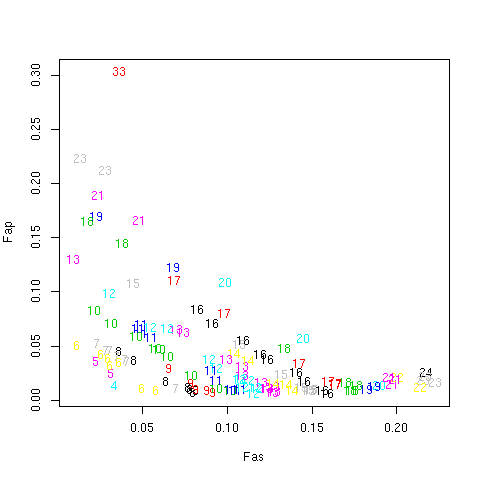
\includegraphics[width=0.9\textwidth]{fasfap.png}
%  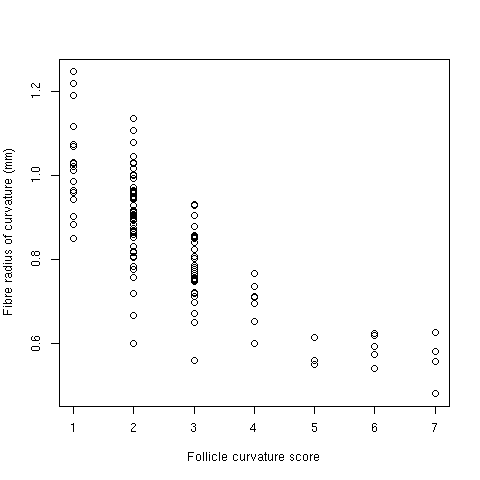
\includegraphics{ofdamm.png}
  \caption{Plot of flock means for area of secondary follicle tissue per $mm^{2}$ of skin against area of primary follicle tissue per $mm^{2}$ of skin for the 126 flocks sampled by Carter(1968)~\cite{cart:68}. The numbers representing each point are the total amount of follicle tissue per $mm^{2}$ of skin as a percentage.}
  \label{fig:fasfap}
\end{figure}

%\end{document}

